\mode*

\section{Behållare}

\subsection{Listor}

\begin{frame}[fragile]
  \mintinline[fontsize=\huge,escapeinside=||]{python}{var = [item0, |$\dotsc$|, itemN]}
\end{frame}

\begin{frame}[fragile]
  \begin{example}
    \begin{minted}{python}
names = ["Adam", "Bertil", "Cesar"]
print(names[0])
print(names[1])
print(names[2])
print(names[3])
    \end{minted}
  \end{example}

  \pause

  \begin{example}
    \begin{minted}{python}
numbers = [2, 3, 12, 3, 12, 12]
print(numbers[0])
print(numbers[1])
print(numbers[2])
    \end{minted}
  \end{example}
\end{frame}

\begin{frame}[fragile]
  \begin{example}
    \begin{minted}{python}
names = ["Adam", "Bertil", "Cesar"]
names[0] = "Ada"
names[1] = "Beda"
names[2] = "Cissi"
print(names[0])
print(names[1])
print(names[2])
names[3] = "Diddi"
    \end{minted}
  \end{example}
\end{frame}

\begin{frame}
  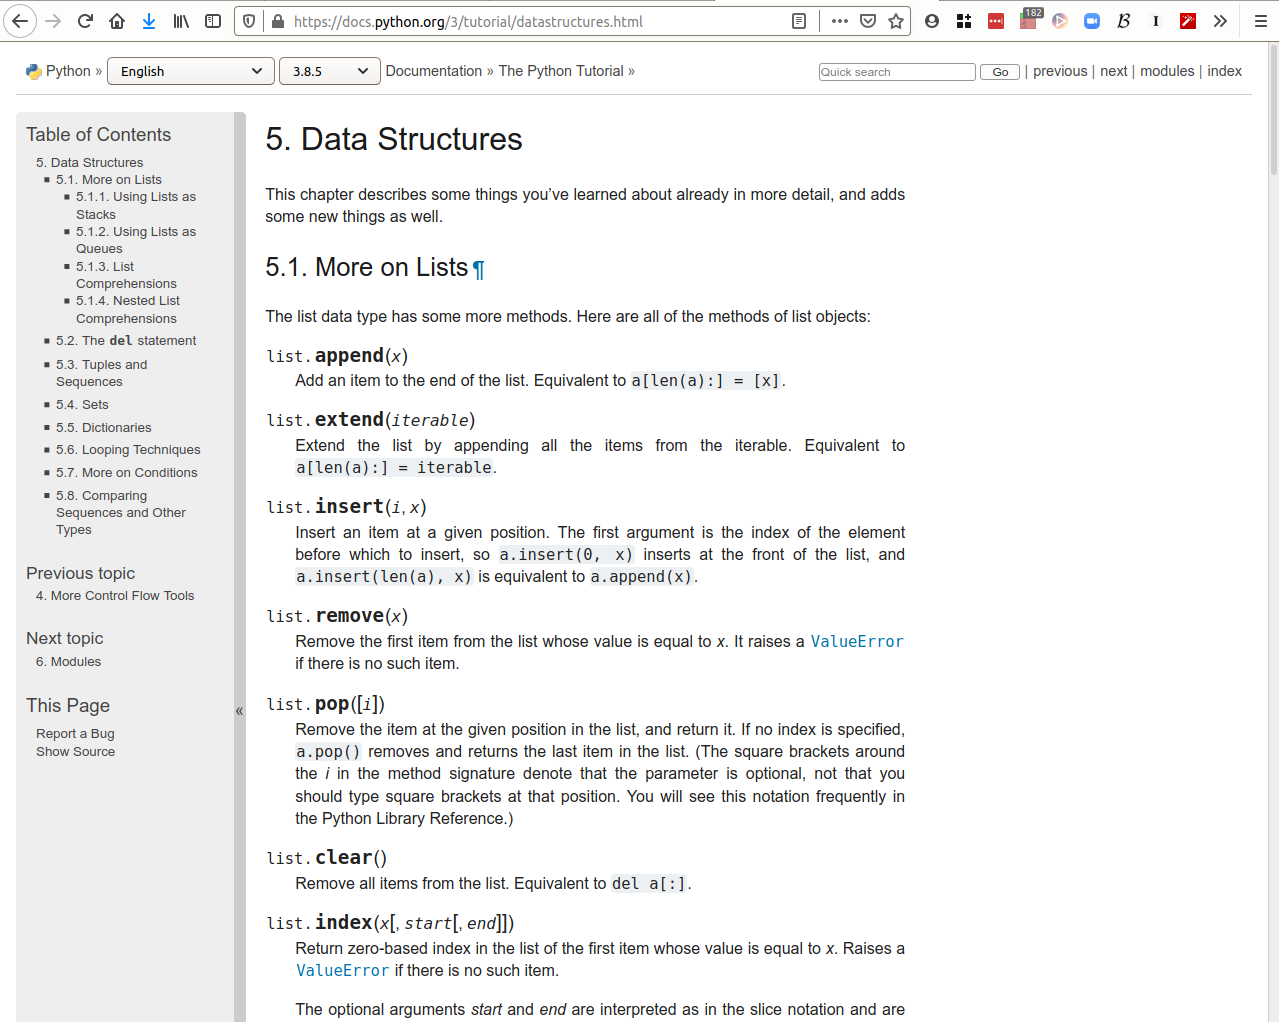
\includegraphics[width=\columnwidth]{figs/docs-lists.png}
\end{frame}

\begin{frame}[fragile]
  \begin{example}[extend\textunderscore{}lists.py]
    \inputminted{python}{examples/extend_lists.py}
  \end{example}
\end{frame}

\begin{frame}[fragile]
  \begin{example}[Aritmetiska \emph{hel}talsföljder]
    \begin{minted}{python}
print(list(range(10)))
print(list(range(0, 10)))
print(list(range(1, 10, 2)))
    \end{minted}
  \end{example}
\end{frame}

\begin{frame}[fragile]
  \mintinline[fontsize=\huge]{python}{var = [f(x) for x in lst]}
\end{frame}

\begin{frame}[fragile]
  \begin{example}[List comprehensions]
    \begin{minted}{python}
squares = [x**2 for x in range(10)]
    \end{minted}
  \end{example}

  \pause

  \begin{example}[List comprehensions]
    \begin{minted}{python}
names = ["anna", "cissi"]
names_capitalized = [name.capitalize() for name in names]
    \end{minted}
  \end{example}
\end{frame}


\subsection{Sökning}

\begin{frame}[fragile]
  \mintinline[fontsize=\huge]{python}|item in list|
\end{frame}

\begin{frame}[fragile]
  \begin{example}[isin.py]
    \inputminted{python}{examples/isin.py}
  \end{example}
\end{frame}

\begin{frame}[fragile]
  \begin{exercise}[search.py]
    \begin{itemize}
      \item Skriv ett program som låter oss mata in ett antal 
        namn.
      \item Därefter får vi söka bland namnen.
    \end{itemize}
  \end{exercise}
\end{frame}

\begin{frame}[fragile]
  \begin{exercise}[search.py]
    \begin{itemize}
      \item Skriv ett program som låter oss mata in ett antal 
        namn.
      \item Därefter får vi söka bland namnen.
    \end{itemize}
  \end{exercise}

  \begin{exercise}[partial\textunderscore{}search.py]
    \begin{itemize}
      \item Ändra programmet så att vi kan söka efter delar av namn.
%      \item Tips: testa hur \mintinline{python}|in| funkar på strängar; 
%        \mintinline{python}|"kaka" in "pepparkaka"|.
    \end{itemize}
  \end{exercise}
\end{frame}

\subsection{Sortering}

\begin{frame}[fragile]
  \begin{example}[Sortering]
    \begin{minted}{python}
      names = ["Beda", "Ada", "Cissi"]
      print(sorted(names))
    \end{minted}
  \end{example}

  \begin{exercise}[Från OLI]
    \begin{itemize}
      \item Vad är förväntat resultat och varför?
    \end{itemize}
    \begin{minted}{python}
numbers = ["2", "1", "3"]
print(sorted(numbers))

numbers.extend(["13", "12", "11"])
print(sorted(numbers))
    \end{minted}
  \end{exercise}
\end{frame}


\subsection{Stackar och köer}

\begin{frame}[fragile]
  \begin{example}[pile.py]
    \inputminted{python}{examples/pile.py}
  \end{example}
\end{frame}

\begin{frame}[fragile]
  \begin{example}[queue.py]
    \inputminted{python}{examples/queue.py}
  \end{example}
\end{frame}

\begin{frame}
  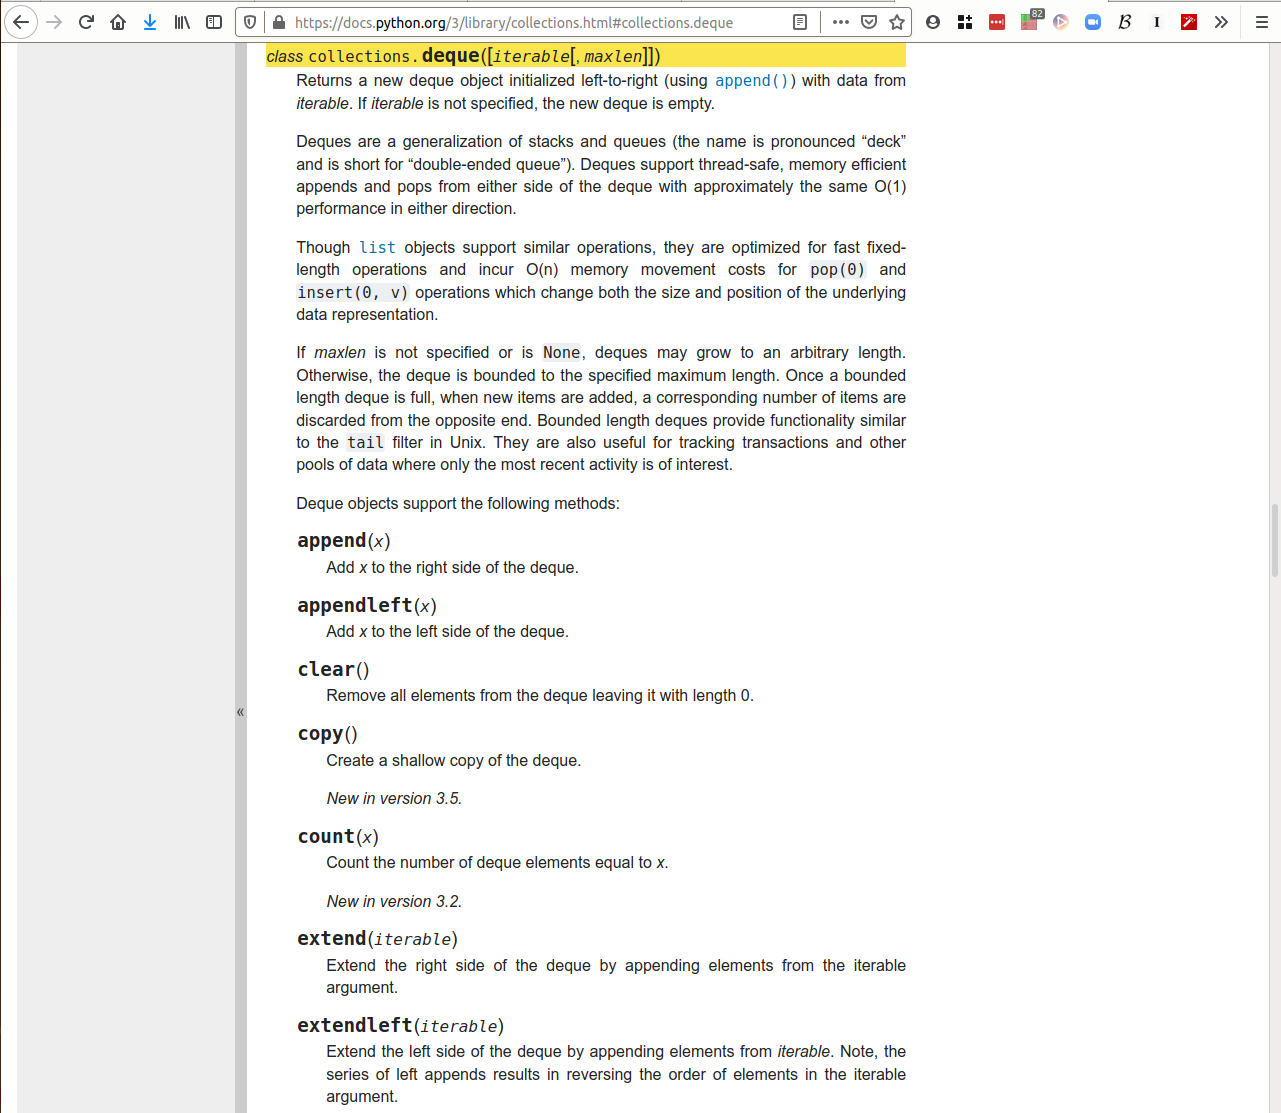
\includegraphics[width=\columnwidth]{figs/docs-deque.png}
\end{frame}

\begin{frame}[fragile]
  \begin{exercise}
    \begin{itemize}
      \item Skriv ett förbättrat program för att diska.
      \item Vi hade diska.py, vill ha dishwasher.py.
    \end{itemize}
  \end{exercise}
\end{frame}


\subsection{Mängder}

\begin{frame}[fragile]
  \begin{example}[sets.py]
    \inputminted{python}{examples/sets.py}
  \end{example}
\end{frame}


\subsection{Uppslagslistor}

\begin{frame}
  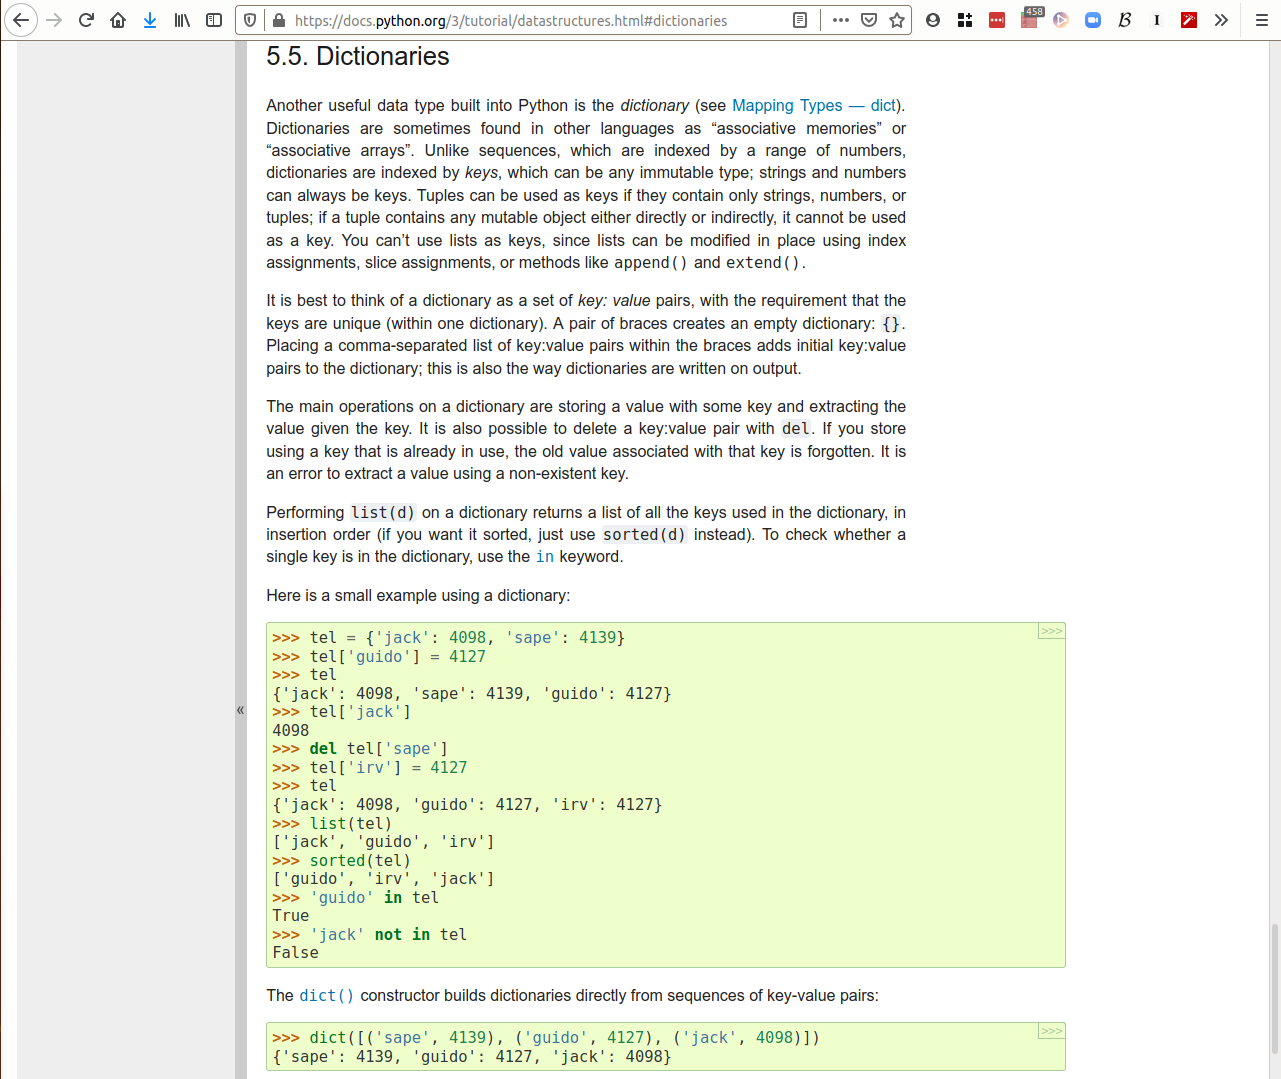
\includegraphics[width=\columnwidth]{figs/docs-dicts.png}
\end{frame}

\begin{frame}[fragile]
  \begin{example}[phone-small.py]
    \inputminted{python}{examples/phone-small.py}
  \end{example}
\end{frame}


\section{Iterationer med for-slingor}

\subsection{For-slingan}

\begin{frame}[fragile]
  \begin{minted}[fontsize=\huge,numbers=none]{python}
for item in container:
  print(item)
  \end{minted}
\end{frame}

\begin{frame}[fragile]
  \begin{example}
    \begin{minted}{python}
for i in range(10):
  print(i)
    \end{minted}
  \end{example}
\end{frame}

\begin{frame}[fragile]
  \begin{example}
    \begin{minted}{python}
for person in ["adam", "bertil", "cesar"]:
    print(person)
    \end{minted}
  \end{example}
\end{frame}

\begin{frame}[fragile]
  \begin{example}[phone-for.py]
    \inputminted{python}{examples/phone-for.py}
  \end{example}
\end{frame}



\section{Tupplar}

\begin{frame}[fragile]
  \begin{example}[tuples.py]
    \inputminted{python}{examples/tuples.py}
  \end{example}

  \pause

  \begin{example}
    \begin{minted}{python}
def my_enumerate(iterable):
  """Returnerar en lista med (n, item) där item är element i iterable."""
  result = []

  for i in range(len(iterable)):
    result.append((i, iterable[i]))

  return result
    \end{minted}
  \end{example}
\end{frame}

\begin{frame}[fragile]
  \begin{example}[fullname.py]
    \inputminted[firstline=3,lastline=7]{python}{examples/fullname.py}
  \end{example}

  \pause

  \begin{example}[fullname-alt.py]
    \inputminted[firstline=3,lastline=7,highlightlines=7]{python}{examples/fullname-alt.py}
  \end{example}
\end{frame}

\begin{frame}[fragile]
  \begin{exercise}
    \begin{itemize}
      \item Vad är skillnaden mellan en lista och en tuppel?
      \item \mintinline{python}|a = [1, 2, 3]|
      \item \mintinline{python}|b = (1, 2, 3)|
    \end{itemize}
  \end{exercise}
\end{frame}


\section{Större exempel}

\begin{frame}
  \begin{exercise}[Snygga utskrifter, align.py]
    \begin{itemize}
      \item Skriv en funktion som skriver ut element snyggt på rader.
    \end{itemize}
  \end{exercise}
\end{frame}

\begin{frame}
  \begin{exercise}[Telefonbok, phone-big.py och phonebook.py]
    \begin{itemize}
      \item Skriv ett program som fungerar som telefonkatalog (hitta.se eller 
        eniro.se?)
      \item Skriv ut alla i alfabetisk ordning.
      \item Låt användaren därefter skriva vems telefonnummer hen vill se.
    \end{itemize}
  \end{exercise}
\end{frame}

\begin{frame}
  \begin{exercise}[Svårare gissningar, guess.py]
    \begin{itemize}
      \item Skriv ett gissningsprogram.
      \item Programmet ska komma ihåg hur många försök som krävdes på varje 
        fråga.
      \item I slutet räknas medelantalet försök ut.
    \end{itemize}
  \end{exercise}
\end{frame}

